\documentclass{article}
\usepackage{pgf,tikz,tikzscale} 
\usepackage{amssymb}
\usepackage{tcolorbox}
\usepackage{xcolor}
\usepackage[utf8]{inputenc}
\usepackage[english]{babel}
\usepackage{multicol}
\usepackage{enumerate}	
\usepackage{graphicx,lipsum,pgfplots} 
\usepackage{amsmath, amsthm}                 
\usepackage[top=1in,bottom=1in, left=.5in, right=.5in] {geometry}  
\usepackage{fancyhdr}       



\pagestyle{fancy}              
\lhead{Math 5910 \newline HW: 2.5-2.6}   
\rhead{Warren Keil}







\begin{document}
\setlength{\parindent}{0cm}   %%%%%%%% KEEP THIS  for block style para. 



%%%%%%%%%%%%%%%%%        1   %%%%%%%%%%%%%%%%%%%%
\textbf{Section 2.5}

\textbf{1.}  Write a formula for the solution to the problem
\begin{align*}
u_{tt}-c^2u_{xx} &= \sin x,  \hspace{2mm} x\in \mathbb{R}, \hspace{2mm} t>0, \\
u(x,0) = u_t(x,0) &= 0, \hspace{2mm} x\in \mathbb{R}.
\end{align*}
Graph the solution surface when \(c=1\). 


\vspace{3mm}
\textit{Solution.} First, let \(w(x,t;\tau) \) be a solution to the following: 
\begin{align*}
 w_{tt} - c^2w_{xx} &= 0 , \hspace{2mm} x \in \mathbb{R} \hspace{2mm} t>0, \\
 w(x,0;\tau) &=0, \hspace{2mm} x \in \mathbb{R}, \\
 w_t(x,0,\tau) &= \sin(x;\tau), \hspace{2mm} x \in \mathbb{R}.
\end{align*}
By d'Alembert's formula in section 2.2, we know that \(w\) has the form, 
\[
w(x,t,\tau) = \frac{1}{2c} \int_{x-ct}^{x+ct} \sin(s;\tau) ds. 
\]
Hence, by Duhamel's Principal, we know that \(u\) has the form, 
\begin{align*}
u(x,t) &= \frac{1}{2c} \int_0^t \int_{x-c(t-\tau)}^{x+c(t-\tau)} \sin(s,\tau) ds d\tau \\
&= \frac{1}{2c} \int_0^t \cos(x-ct+c\tau)) - \cos(x+ct -c\tau)   d\tau  \\
&= \frac{1}{2c} \left( \frac{1}{c} \sin(x-ct+ct) -  \frac{1}{-c}   \sin(x+ct-ct) -  \frac{1}{c}\sin(x-ct) +\frac{1}{-c} \sin(x+ct)  \right) \\
&= \frac{1}{2c^2} ( \sin(x) + \sin(x) - \sin(x+ct) -\sin(x-ct) ) \\
&= \frac{1}{c^2} \sin(x) - \frac{1}{2c^2} \sin(x+ct)+  \frac{1}{2c^2} \sin(x-ct).
\end{align*}


\begin{flushright}
\( \qed \)
\end{flushright}
We use the following python code to plot the 3d surface of this solution when \(c=1\). 
\begin{multicols}{2}
\begin{verbatim}
x = np.arange(-10, 10, .05)
t = np.arange(0, 20, .05)
x, t = np.meshgrid(x, t)
u = np.sin(x) - .5*np.sin(x+t) - .5*np.sin(x-t)

# Plot the surface.
surf = ax.plot_surface(x, t, u, cmap=cm.coolwarm,
                       linewidth=0, antialiased=False)

# Customize the z axis.
ax.set_zlim(-1.5, 3.5)
ax.zaxis.set_major_locator(LinearLocator(10))
ax.zaxis.set_major_formatter(FormatStrFormatter('%.02f'))

# Add a color bar which maps values to colors.
fig.colorbar(surf, shrink=0.5, aspect=5)

plt.show()
\end{verbatim}

\begin{flushright}
\includegraphics[scale=.65]{pde_2p5_plot}
\end{flushright}
\end{multicols}
\newpage
%%%%%%%%%%%%%%%%%        4   %%%%%%%%%%%%%%%%%%%%
\textbf{4.} Formulate Duhamel's principle and solve the initial boundary value problem 
\begin{align*}
u_{t} &= ku_{xx} + f(x,t),  \hspace{2mm} x>0, \hspace{2mm} t>0, \\
u(x,0) &=0, \hspace{2mm} x>0, \\
u(0,t) &= 0, \hspace{2mm} t>0. 
\end{align*}
 The solution is
 \[
 u(x,t) = \int_0^t \int_0^\infty (G(x-y,t-\tau) - G(x+y,t-\tau))f(y,\tau)dyd\tau.
 \]

\vspace{3mm}
\textit{Solution.} We first notice that this is a non-homogeneous diffusion PDE with a source on a semi-definite spatial domain and with zero values for the initial and boundary conditions. First, we will use Duhamel's Principal to transform this PDE to a homogeneous one. Let \(w(x,t;\tau)\) be a solution to the following,
\begin{align*}
w_t &= kw_{xx}, \hspace{2mm} x>0, \hspace{2mm} t>0, \\
w(x,0) &= f(x,\tau), \hspace{2mm} x>0, \\
w(0,t) &= 0 \hspace{2mm} t>0.
\end{align*}
Next, since we are on a semi-infinite domain, then by section 2.4 and on pg. 97, we know \(w\) has the form
\[
w(x,t;\tau)= \int_0^{\infty} [G(x-y,t) - G(x+t,t)] f(y,\tau) dy , \hspace{2mm} x \geq 0. 
\]
\textit{(where G is Green's function) }
Now using Duhamel's Principal, we get that, 
\[
u(x,t) = \int_0^t \int_0^{\infty} [G(x-y,t-\tau) - G(x+y,t-\tau)] f(y,\tau) dy d\tau.
\]
\begin{flushright}
\( \diamondsuit \)
\end{flushright}



\newpage
%%%%%%%%%%%%%%%%%        1   %%%%%%%%%%%%%%%%%%%%
\textbf{Section 2.6}

\textbf{1.}Solve the following using Laplace transforms. 
\begin{align*}
u_{tt} &= c^2u_{xx} - g,  \hspace{2mm} x>0, \hspace{2mm} t>0, \\
u(0,t) &=0, \hspace{2mm} t>0, \\
u(x,0) &= u_t(x,0) = 0, \hspace{2mm} x>0. 
\end{align*}
The solution shows what happens to a falling cable lying on a table that is suddenly removed. Sketch some time snapshots of the solution. 


\vspace{3mm}
\textit{Solution.} We begin by taking the Laplace transform of both sides of the PDE, (for the rest of this paper, we denote \(\mathcal{L} [ u(x,t) ] = U(x,s) = \int_0^{\infty} u(x,t)e^{-st} dt )\). Also before we begin computation, we notice that the problem gives us just \(g\) for a non-homogenous term. Since this model describes something falling, we know that \(g\) is the acceleration due to gravity. \(\frac{9.8m}{s^2}.\)
\begin{align*}
&& \mathcal{L}[ u_{tt} ]&= \mathcal{L} [c^2u_{xx} - f(x,t)],  \hspace{2mm}, x>0, \hspace{2mm} t>0,  &&\\
\hspace{17mm}&& s^2 U(x,s) - su(x,0)-u_t(x,0) &= c^2U_{xx} - \frac{g}{s} && \\
&& s^2 U(x,s)  &= c^2U_{xx} -\frac{g}{s}   &\text{by initial conditions, }u(x,0) &= u_t(x,0) = 0&  \\
&&U_{xx} - \frac{s^2}{c^2} U      &= \frac{g}{sc^2}      &\text{ by  algebra}& \\
\end{align*}
By method of undetermined coefficients (pg. 283), we find that \(U\) has the form,

\[
U(x,s) = c_1(s) U_1(x,s) + c_2(s) U_2(x,s)+ U_p(x),
\]
where \(U_1, U_2\) solve the associated homogenous problem. 
We solve the homogeneous problem by the characteristic equation method, \(m^2 = \frac{s^2}{c^2}\). \( \Rightarrow  m = \pm s/c \). Thus the form of the solution to the homogenous problem is, 
\[
U(x,s) = c_1(s) e^{\frac{sx}{c}} + c_2(s) e^{\frac{-sx}{c}} 
\]
And since only a bounded solution will be sensible, we take \(c_1(x) = 0\). Next, to solve to \(U_p(x,s)\), we make the following initial guess \(U_p(x,s) = A \). Then \( U_{px}=0,\) and \(  U_{pxx}=0.  \) .  So \(U_{pxx} - \frac{s^2}{c^2} U_p= \frac{g}{sc^2} \) becomes: \( 0 - \frac{s^2}{c^2} A = \frac{g}{sc^2}\). Therefore, \(U_p = A = -\frac{g}{s^3} \). Now that we have the particular solution, we can take the Laplace transform of the boundary condition to solve for \(c_2(s)\):
\begin{align*}
\mathcal{L}[ u(0,t)]&= \mathcal{L}[0], t>0  \\
U(0,s) &= 0 = c_2(s)e^0 - g/s^3 \\
c_2(s) &= +g/s^3
\end{align*}

Thus have now have our final solution in the \(x,s\) domain. 
\[
U(x,s) = g/s^3 e^{-sx/c} - g/s^3.
\]
Thus to find \(u\), we take the inverse Laplace transform using the convolution theorem, 
\begin{align*}
u(x,t) = \mathcal{L}^{-1} [U] &= \mathcal{L}^{-1}[ (\frac{2g}{2s^3 } )(e^{-sx/c}) -\mathcal{L}^{-1}[g/s^3]\\
&= \int_0^t ( \frac{g(t-\tau)^2}{2 } )( \delta(\tau- x/c) d\tau  - \frac{ gt^2 }{2}
\end{align*}

\newpage
We now enter our function into mathematica and observe the 3D plot to gain intuition about the solution and we also plot various time snapshots. 

\begin{verbatim}
u[x_, t_] :=  Integrate[ (9.8 (t - h)^2 /2)* DiracDelta[h - x]   , {h, 0, t}] + (9.8/2)*t^2 
Plot3D[u[x, t] , {x, -5, 5}, {t, 0, 10} ]
\end{verbatim}

\begin{centering}
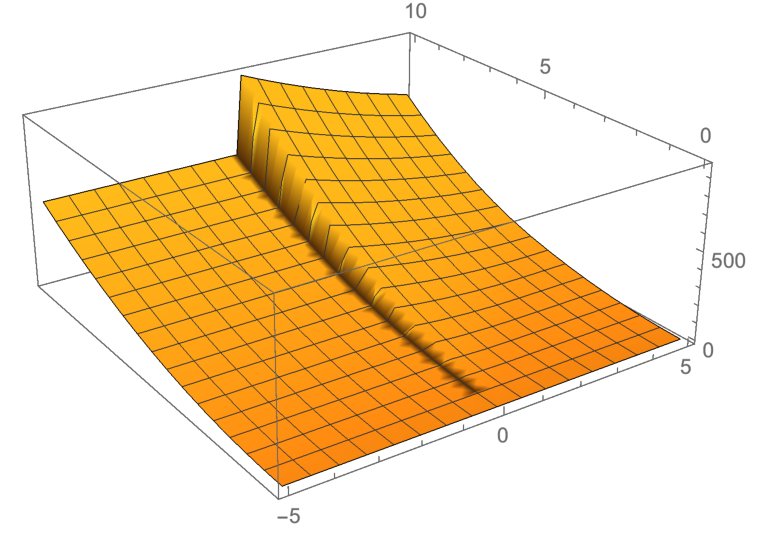
\includegraphics{pde2p63dplot}
\end{centering}

\begin{verbatim}
Plot[ {u[x, .001], u[x, .05], u[x, .1], u[x, .5], u[x, 1], u[x, 2]}, {x, -2, 2}, PlotRange -> All , 
 PlotLegends -> {"t=.001", "t=.0\.105", "t=.1", "t=.5", "t=1",  "t=2"}] 
\end{verbatim}

\begin{centering}
\includegraphics{pde2p62dplot}
\end{centering}

Note: The legend did not save with the rest of the image. The smallest value of \(t\) is the highest line and they follow in order. 
\newpage
%%%%%%%%%%%%%%%%%        2   %%%%%%%%%%%%%%%%%%%%

\textbf{2.} In the quarter plane \(x,y>0\), where the temperature is initially zero, heat flows only in the \(y\)-direction; along the edge \(y=0\) heat is convected along the \(x\)-axis, and the termperature is constantly 1 at the point \(x=y=0\). The boundary value problem for the temperature \(u(x,y,t) \) is 
\begin{align*}
u_t&=u_{yy}, \hspace{2mm} x,t,y>0, \\
u(x,y,0)&= 0 , \hspace{2mm} x,y>0 \\
u(0,0,t)&= 1, \hspace{2mm} t>0,\\
u_t(x,0,t)+ u_x(x,0,t) &= 0, \hspace{2mm}  x,t>0. 
\end{align*}

Find a bounded solution using Laplace transforms. 

\vspace{3mm}
\textit{Solution.} We start by taking Laplace transforms of both sides of the equation. 

\begin{align*}
\mathcal{L}[u_t] &= \mathcal{L}[u_{yy}] \\
sU - u(x,y,0) &= U_{yy} \\
sU &= U_{yy} \\
U_{yy} - sU &=0 
\end{align*}
Now we solve by solving the characteristic equation:
\begin{align*}
m^2-s &=0  \\
m &= \pm \sqrt{s}   \\
\Rightarrow U(x,y,s) &= a(x,s) e^{\sqrt{s}y} + b(x,s)e^{-\sqrt{s}y} 
\end{align*}
Since we only care about bounded solutions, then we can set \( a(x,s) = 0 \). Thus, we have
\[
U(x,y,s) = b(x,s)e^{-\sqrt{s}y}. 
\]
We then solve for \(b(x,s)\) by taking the Laplace transform of the boundary condition of \(y\). 
\begin{align*}
\mathcal{L}[u_t(x,0,t)] + \mathcal{L}[u_x(x,0,t)] &= \mathcal{L}[0] \\
sU(x,0,s) -u(x,0,0) + U_x(x,0,s) &= 0  \hspace{15mm} \text{now plug in out solution for } U\\
sb(x,0)e^0 + \frac{\partial}{\partial x} b(x,0)e^0 &= 0  \\
\frac{\partial}{\partial x} b(x,0) + sb(x,0)  &=0     \hspace{15mm} \text{ rearranging} \\
\int \frac{\partial}{\partial x} b(x,0)\cdot e^{sx} dx &= \int dx \text{ solving with ODE method, IF}\\ 
b(x,0) &= e^{-sx} f(s) 
\end{align*}
So far we have used the boundary condition to show that 
\[
U(x,y,s) = f(s) e^{-sx} e^{-\sqrt{s} y}.
\]
We now take the Laplace transform to of \(u(0,0,t)=1 \) to solve for \(f(s)\). 
\begin{align*}
\mathcal{L}[u(0,0,t)=1] &= \mathcal{L}[1] \\
U(0,0,s) = 1/s &= f(s) 
\end{align*}
Thus our solution in terms of \(U\) is \( U(x,y,s)= (1/s)e^{-sx} e^{ -\sqrt{s} y}\).
Thus, \[ 
u(x,y,t) = \mathcal{L}^{-1}[U(x,y,s)]=\mathcal{L}^{-1}[ \left(s^{-1}e^{ -\sqrt{s} y}\right) \cdot \left( e^{-sx}  \right)]=\int_0^t \delta(t-\tau-x) (1-\text{erf}(\frac{y}{2\sqrt{\tau}} ) d\tau 
\]









\end{document}